\documentclass{article}

\usepackage[utf8]{inputenc}
\usepackage[english]{babel}
\usepackage{graphicx}
\usepackage{url}

\graphicspath{ {images/} }

\title{BDI4JADE Tutorial}
\author{Matheus Dias and Ingrid Nunes}
\date{\today}

\begin{document}

\maketitle

\tableofcontents

\newpage

\section{Introduction}\label{sec:introduction}

BDI4JADE\footnote{\url{http://inf.ufrgs.br/prosoft/bdi4jade}} is an agent platform that implements the (belief-desire-intention) (BDI) \cite{Rao:AAMAS1995:BDIArch} architecture. It consists of a BDI layer implemented on top of JADE\footnote{\url{http://jade.tilab.com/}} \cite{Bellifemine:book2007:JADE}. BDI4JADE leverages all the features provided by JADE and reuses it as much as possible. Other highlights of our JADE extension, besides providing BDI abstractions and the reasoning cycle, include:

\begin{itemize}

    \item \textbf{Use of Capabilities} --- agents aggregate a set of capabilities, which are a collection of beliefs and plans, and allow modularisation of particular agent functionality.

    \item \textbf{\texttt{PlanBody} is an Extension of JADE \texttt{Behaviour}} --- in order to better exploit JADE features, plan bodies are subclasses of JADE behaviours.

    \item \textbf{Java Annotations} --- annotations are provided to allow easier configuration of agent components, without compromising its flexibility.

    \item \textbf{Extension Points} --- strategies can be easily implemented to extend parts of the reasoning cycle, such as  belief revision and plan selection.

    \item \textbf{Listeners and Events} --- different events (such as events related to goals and beliefs) can be observed in the platform, allowing listeners to react according to events that occurred.

    \item \textbf{Java Generics for Beliefs} --- beliefs can store any kind of information and are associated with a name, and if the value of a belief is retrieved, it must be cast to its specific type, so the use of Java generics allows us to capture incorrect castings at compile time.

\end{itemize}

As opposed to different BDI platforms that have been proposed, it does not introduce a new programming language nor rely on a domain-specific language (DSL) written in terms of XML files. Because agents are implemented with the constructions of the underlying programming language, Java, we bring two main benefits. First, features of the Java language, such as annotations and reflection, can be exploited for the development of complex applications. Second, it facilitates the integration of existing technologies, e.g.\ frameworks and libraries, which is essential for the development of large scale enterprise applications, involving multiple concerns such as persistence and transaction management. This also enables a smooth adoption of agent technology.

\section{The \texttt{HelloWorld} Application}\label{section:helloWorld}

In this section, we explain details of how the \texttt{HelloWorld} application is implemented. There are two versions of it. The first, detailed in Section~\ref{sec:hwAgent}, is implemented as an agent. The second, described in Section~\ref{sec:hwCapability}, is implemented as a capability, which can be associated with any agent. In order to run these, and other provided examples, you should run the \texttt{BDI4JADEExamplesApp} class.

\subsection{Alternative 1: \texttt{HelloWorldAgent}}\label{sec:hwAgent}

The \texttt{HelloWorld} is an application in which an agent has the goal of saying hello world, and a plan that can achieve it by printing in the main console ``Hello World, \emph{name}!,'' where \emph{name} is given as parameter of the agent goal.

Agents in BDI4JADE are associated with a single or multiple capabilities. The agent that is part of the \texttt{HelloWorld} application has a single capability, and is implemented in the class \texttt{HelloWorldAgent}, which extends the \texttt{SingleCapabilityAgent}. Alternatively, you may create an agent that may be associated with multiple capabilities. In this case, instated of extending \texttt{SingleCapabilityAgent}, you must extend \texttt{MultipleCapabilityAgent}.

\begin{figure}[!h]
\centering

\includegraphics[width=\linewidth]{agentdecl}
\label{fig:agentdecl}
\end{figure}

Goals may be added to agents, which in BDI4JADE are objects that are instance of any Java class that implements the \texttt{Goal} interface. In our example, the goal of saying hello world is implemented in the inner class \texttt{HelloWorldGoal}, whose enclosing class is the \texttt{HelloWorldAgent} class. \texttt{HelloWorldGoal} has a single constructor of receives a parameter that indicates the name that should be used in the hello world message. This parameter may be later retrieved by a getter.

\begin{figure}[!h]
\centering
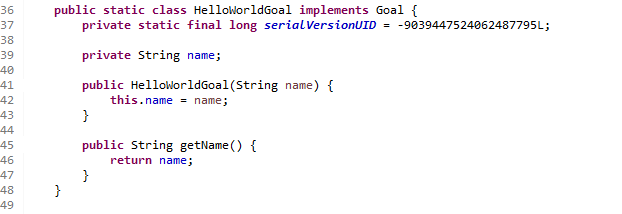
\includegraphics[width=\linewidth]{AgentGoal}
\label{fig:agentGoal}
\end{figure}

In order for an agent to be able to achieve this goal, it must have a plan that achieves it. A plan has some informational details about it, such as a template that specifies which goals it can achieve, and a body.  In our example, a plan body is implemented in the \texttt{HelloWorldPlanBody} class, which extends the \texttt{AbstractPlanBody} class and is also implemented as an inner class of the \texttt{HelloWorldAgent} class. The implementation of the \texttt{action()} method consists of printing the hello world message and then setting the end state of the plan as successful (\texttt{EndState.SUCCESSFUL}).

\begin{figure}[!h]
\centering
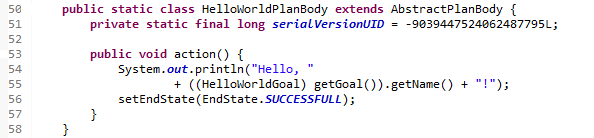
\includegraphics[width=\linewidth]{helloplan}
\label{fig:helloplan}
\end{figure}

The method \texttt{getGoal()} (part of the \texttt{PlanBody} interface implemented by the \texttt{AbstractPlanBody} class) returns the goal that triggered the execution of the plan, and in this case we know it is an instance of \texttt{HelloWorldGoal} class. So, to get the parameter of the goal to print the hello world message, we invoke the \texttt{getGoal()} method, cast its return to \texttt{HelloWorldGoal}, and get its parameter by invoking the \texttt{getName()} method.

Given that we now have a plan body --- the \texttt{HelloWorldPlanBody} --- we need to create a \texttt{Plan} and add it to the agent. This is done in the constructor of the \texttt{HelloWorldAgent} class. The default constructor of the  \texttt{SingleCapabilityAgent} class (which is the \texttt{HelloWorldAgent} parent class) is implicitly invoked in the \texttt{HelloWorldAgent} constructor. This implicitly invoked constructor instantiates a \texttt{Capability} and associates it with the agent. This \texttt{Capability} can be accessed by the \texttt{getCapability()} method. Capabilities are associated with a plan library, accessed by the \texttt{getPlanLibrary()} method, which has the method \texttt{addPlan()}, which in turn adds a plan to the capability plan library. So in the \texttt{HelloWorldAgent} constructor, we add a plan that is an instance of \texttt{DefaultPlan} class to the capability plan library. This class has a constructor that receives as a parameters (i) a class of goals that can be achieved by the plan; and (ii) a class that implements \texttt{PlanBody}. Therefore, in our case, we instantiate the \texttt{DefaultPlan} with the goal class \texttt{HelloWorldGoal}, and plan body class \texttt{HelloWorldPlanBody}.

\begin{figure}[!h]
\centering
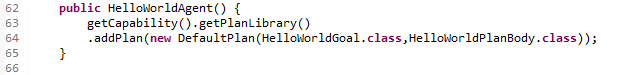
\includegraphics[width=\linewidth]{helloConstr}
\label{fig:helloConstr}
\end{figure}

The \texttt{HelloWorldAgent} can be instantiated and executed like any JADE agent. After the \texttt{HelloWorldAgent} is started, an instance of the \texttt{HelloWorldGoal} must be added to the agent by invoking the method \texttt{addGoal()}, in order to the agent try to, and eventually achieve, this goal.

\subsection{Alternative 2: \texttt{HelloWorldAnnotatedCapability}}\label{sec:hwCapability}

The previous section showed how to create an agent, without creating a capability separately. In this section, we detail an alternative implementation of the \texttt{HelloWorld} application, which consists of a capability that can be added to agents, taking advantage of the BDI4JADE annotations.\footnote{\url{http://docs.oracle.com/javase/tutorial/java/annotations/}} The created capability is the \texttt{HelloWorldAnnotatedCapability} class, which extends the \texttt{Capability} class.

\begin{figure}[!h]
\centering

\includegraphics[width=\linewidth]{capability}
\label{fig:capability}
\end{figure}

Simular to the previous version of the \texttt{HelloWorld} application, there is an inner class that represents the goal to be achieved --- the \texttt{HelloWorldGoal}.

\begin{figure}[!h]
\centering
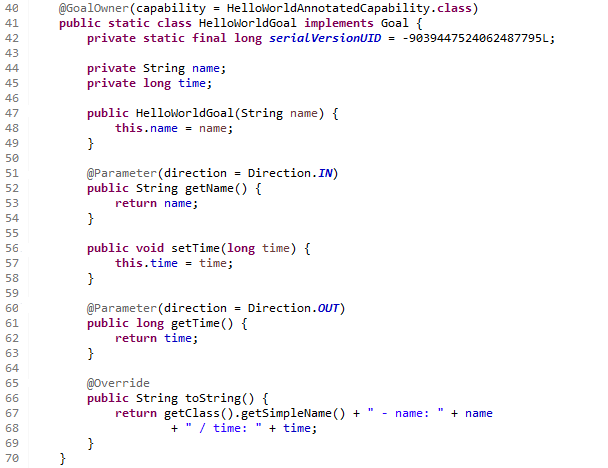
\includegraphics[width=\linewidth]{hellogoaal}
\label{fig:hellogoal}
\end{figure}

This goal was implemented with additional features. We used the \texttt{@GoalOwner} annotation to indicate to which capability this goal belongs and, given that we do not specify whether this goals is external or internal, it is considered \emph{external} because it is the default value. The consequence of having a goal owner is that this goal can be achieved only by the capability to which it belongs (or part or child capabilities). For further information about it, we refer the reader to elsewhere~\cite{Nunes:EMAS2014:CapabilityRelationships,Nunes:EMAS2014PostProc:CapabilityRelationships}.

Besides using the \texttt{@GoalOwner} annotation, we used the \texttt{@Parameter} annotation to indicate goal parameters. There is one input parameter (\texttt{Direction.IN}), which is the \emph{name} to be displayed in the hello world message. It is specified in the goal constructor and can be retrieved by a getter. In addition, there is an output parameter (\texttt{Direction.OUT}) named \emph{time}, which will be set with the time when the hello world message is displayed. The time parameter has both a setter, to be used by the plan body that achieves this goal to set its value, and a getter, used to get this value afterwards.

In order to create a plan to achieve the \texttt{HelloWorldGoal}, we also need to create a plan body, whose name is \texttt{HelloWorldPlanBody}, which also extends the \texttt{AbstractPlanBody} class and is also implemented as an inner class of the capability. By using the \texttt{@Parameter} annotation, the plan body can automatically get input parameters and set output parameters. Given that there is a setter of \emph{name}, which is annotated as an input parameter, the value obtained by a getter of \emph{name} from the goal that triggered the plan body execution will be set by invoking this setter, before executing the plan body. Similarly, after the plan body execution, the value obtained by the getter of \emph{time} in the plan body will be used to set the value of the output parameter with the same name of the goal that triggered the plan body. Therefore, based on the annotations, BDI4JADE automatically sets input and output parameters.

\begin{figure}[!h]
\centering
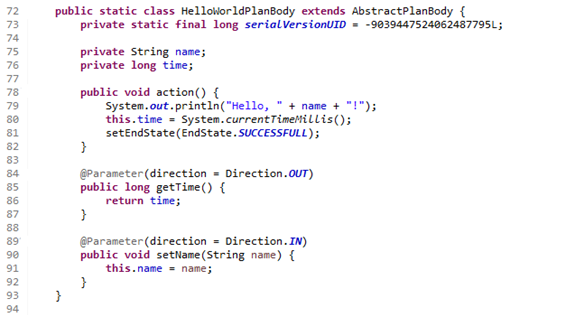
\includegraphics[width=\linewidth]{CapaPlan}
\label{fig:capaplan}
\end{figure}

Finally, to add a plan to a capability using annotations, we add an attribute whose type is \texttt{Plan}, or any class that implements it, to the capability. This attribute should be annotated with the \texttt{@Plan} annotation, as shown below.

\begin{figure}[!h]
\centering

\includegraphics[width=\linewidth]{objplan}
\label{fig:objplan}
\end{figure}

A \texttt{DefaultPlan} is instantiated to initialise the \texttt{plan} attribute. The \texttt{DefaultPlan}  receives as parameter the \texttt{HelloWorldGoal} class and the \texttt{HelloWorldPlanBody} class, indicating that it is a plan that can achieve goals instance of \texttt{HelloWorldGoal} and, to do so, the plan body \texttt{HelloWorldPlanBody} must be executed.

The \texttt{HelloWorldAnnotatedCapability} capability can then be instantiated and added to any agent or associated with other capabilities.

\section{BDI4JADE Main Components}\label{sec:components}

\subsection{BDI Agents} \label{sec:BDIagent}

A BDI agent represents an agent that follows the BDI  software model. And have a reasoning cycle, responsible for driving the agent behaviour, strategies, and capabilities.

The agent class must extends the capability, and may have a goal class and a planbody class. The goal class and the planbody class can be declared in the capability.

\begin{figure}[!h]
	\centering
	
\includegraphics[width=\linewidth]{agentdecl}
	\label{fig:agentdecl}
\end{figure}

\subsection{Capabilities} \label{sec:capability}

A capability in BDI4JADE is self-contained in the agente the capability consisting of (i) a set of plans, (ii) a fragment of the knowledge base that is manipulated by these plans and (iii) a specification of the interface to the capability.

\begin{figure}[!h]
	\centering
	
\includegraphics[width=\linewidth]{capability}
	\label{fig:capability}
\end{figure}

\subsection{Goals} \label{sec:goal}

Goals represent the motivational state of the system, and represent desires that the agent wants to achieve.

A goal in BDI4JADE can be any Java object, with the condition that it must implement the Goal interface.the implementation of the goal interface may need the annotation {@link GoalOwner} in order to especify the capability that own this goal.If is required add a new goal to an agent, the only thing that must be done is to invoke the method void addGoal(Goal goal) of an instance of the BDIAgent.

\begin{figure}[!h]
	\centering
	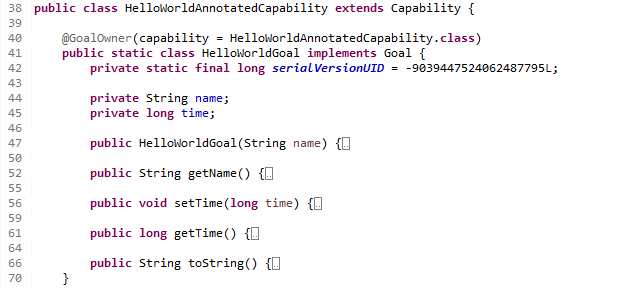
\includegraphics[width=\linewidth]{Goal}
	\label{fig:goal}
\end{figure}

\subsection{Plans} \label{sec:plans}

\subsubsection{Plans}

The representation of plans in BDI4JADE is not associated with one but with a set of classes. This is because our goal is to reuse JADE as much as possible. In the BDI4JADE platform there is three main kind of plans.

Plans do not state a set of actions to be executed to achieve a goal, but have some information about them.Beside this they define the methods that will be implemented by the sub-classes.  

\begin{figure}[!h]
	\centering
	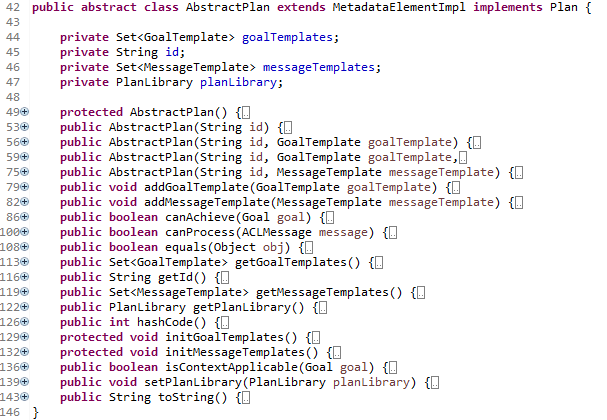
\includegraphics[width=\linewidth]{Plan}
	\label{fig:Plan}
\end{figure}

\subsubsection{Plan Bodies}

Plan bodies must implement the \texttt{PlanBody} interface and extend the JADE \texttt{Behaviour} class. Alternatively, a plan body can simply extend the \texttt{AbstractPlanBody} class. A plan body must implement the method \texttt{action()} that contains actions to achieve goals. To indicate that a plan has completed its execution, the \texttt{setEndState(EndState)} must be invoke, with one of two parameters: (i) \texttt{EndState.SUCCESSFUL}; or (ii) \texttt{EndState.FAILED}. The former indicates that the plan was successfully completed, while the latter indicates that the plan failed. Before the end state of a plan is set, the method \texttt{getEndState()} returns \texttt{null}, meaning that the plan is still being executed.

%The planbody class implements the AbstractPlanBody interface and must own the set of actions to be executed by a plan. Beside this two methods must be implemented the former is EndState getEndState(), returns the end state of the plan body. If it has not finished yet, it should return null. This shows that the platform detects that a goal was achieved when the selected plan finished with a SUCCESSFUL state. 

\begin{figure}[!ht]
	\centering
	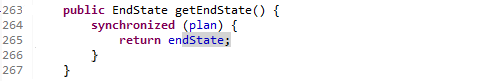
\includegraphics[width=\linewidth]{GetEndState}
	\label{Rotulo}
\end{figure}

The latter is the void init (PlanInstance planinstance), is invoked when the plan body is instantiated. This is used to initialise it, for instance retrieving parameters of the goal to be achieved.

\begin{figure}[!ht]
	\centering
	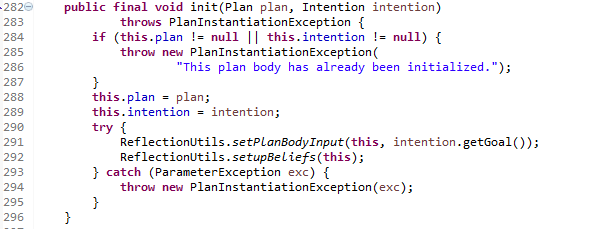
\includegraphics[width=\linewidth]{voidInit}
	\label{fig:voidInit}
\end{figure}

%\textbf{Plans Instances}
%\newline
%Plan instances are created to achieve a particular goal, according to a specification of a plan.
%\newline
%\textbf{Implementation}
%\newline
%The implementation of plan instances requires the following attributes.
%\newline

\begin{description}
	\item[Behaviour behaviour] The behaviour being executed to achieve the goal associated with the intention.
	\item[Intention] The intention whose goal is trying to be achieved.
	\item[Plan plan] The plan that this plan instance is associated with.
	\item[EndState endstate] The end state of the plan instance (FAILED or SUCCESSFUL), or null if it is currently being executed.
	\item[List$\langle$Goal$\rangle$ subgoals] The subgoals dispatched by this plan. In case the goal of the intention associated with the plan of this plan instance is dropped, all subgoals are also dropped.
	\item[List$\langle$GoalFinishedEvent$\rangle$ goalEventQueue] When this plan instance dispatches a goal, it can be notified when the dispatched goal finished.
\end{description}

\bibliographystyle{plain}
\bibliography{tutorial}

\end{document} 